% ==========================================================================
% latency.tex  -  self-contained "Latency and scalability" section.
%
% Generated by scripts/gen_tex.py from scripts/computed_stats.json, which is in
% turn produced by scripts/analysis.py from the logs in new_results/.
% Tables and figures are measured; re-run the two scripts to refresh them.
%
% The document compiles on its own (pdflatex latency.tex). To fold it into the
% MDPI paper, drop the body between \begin{document} and \end{document} into
% Section~\ref{sec:hardwareanalysis} and keep the figures in figures/.
% ==========================================================================
\documentclass[11pt]{article}
\usepackage[a4paper,margin=2cm]{geometry}
\usepackage{graphicx}
\usepackage{booktabs}
\usepackage{array}
\usepackage{float}
\usepackage{caption}
\graphicspath{{../../figures/}{figures/}{../figures/}{./}{../}}
\setlength{\tabcolsep}{4pt}

\begin{document}

\section{Latency and scalability}
\label{subsub:latency}

This section characterises the latency of the leader agent and how it scales. The
end-to-end latency is the time from the reception of a user query to the delivery
of the natural-language reply. Serving a query involves two language-model
invocations on the leader: a \emph{tool-dispatch} stage, which reads the user
query together with the JSON descriptions of the exposed tools and emits one tool
call, and a \emph{final-reply} stage, which turns the returned tool result into a
natural-language answer. For each stage the time to first token (TTFT), which
corresponds to the prefill of the prompt, is reported separately, as it dominates.
Two leader backends are measured: \texttt{Qwen3:1.7b} on the Hailo-10H of the
Raspberry Pi 5 and \texttt{functiongemma:270m} on the CPU of the STM32MP257F-DK.
After the model load time and the effect of the number of agents, latency is
studied along two axes, the number of exposed tools and the number of aggregated
replies. The interpretation of all these measurements is collected in the
Discussion (Subsection~\ref{subsec:latency_discussion}).

\subsection{Model load time}
\label{subsub:latency:boot}

Before serving any query, the leader loads its language model. This cost is paid
once, at agent start-up or immediately after a leader election, and is not part of
the per-query latency. Table~\ref{tab:boot} reports the load time over ten
consecutive loads. Both backends show a one-time cold start on the first load that
is markedly slower than the warm loads, which cluster near the minimum
($3.89$~s for \texttt{functiongemma:270m}, $6.75$~s for
\texttt{Qwen3:1.7b}), while the cold start reaches the maximum ($9.57$~s and
$31.03$~s respectively). The mean and standard deviation are computed over all
ten loads and therefore include this cold-start outlier.

\begin{table}[H]
\centering
\caption{Average model load time (time to load the language model on the leader),
over ten consecutive loads per model. The minimum is a warm load, the maximum a
cold start.}
\label{tab:boot}
\begin{tabular}{llcccc}
\toprule
\textbf{Model} & \textbf{Device (backend)} & \textbf{Mean [s]} & \textbf{Std [s]} & \textbf{Min [s]} & \textbf{Max [s]} \\
\midrule
\texttt{functiongemma:270m} & STM32MP257F-DK (CPU) & 4.47 & 1.79 & 3.89 & 9.57 \\
\texttt{Qwen3:1.7b} & Raspberry Pi 5 (Hailo) & 9.27 & 7.65 & 6.75 & 31.03 \\
\bottomrule
\end{tabular}
\end{table}

\subsection{Agent scaling and network overhead}
\label{subsub:latency:agents}

The cost of scaling the number of agents is considered first, in power and in
network traffic. Table~\ref{tab:power_agents} and Figure~\ref{fig:power_agents}
report the aggregate power consumption of the STM32MP257F-DK as the number of
co-located agents grows from $1$ to $100$, measured on the STM32MP257F-DK board. The
mean power stays close to $4.3$~W throughout, so the asynchronous communication
layer adds no measurable power overhead.

% External tables are kept in graphs/ and pulled in with \input.
% Remove these \input lines when merging into the paper if the tables already exist.
\begin{table}[H]
\caption{Power statistics per number of agents.}
\label{tab:power_agents}
\begin{tabular}{lcccc}
\toprule
 & Min [W] & Mean [W] & Max [W] & Std Dev [W] \\
Section &  &  &  &  \\
\midrule
1 agent & 4.1740 & 4.2936 & 4.4969 & 0.0332 \\
10 agents & 4.1761 & 4.2956 & 4.3877 & 0.0294 \\
20 agents & 4.1765 & 4.2991 & 4.3821 & 0.0264 \\
50 agents & 4.1837 & 4.3021 & 4.4377 & 0.0263 \\
100 agents & 4.1839 & 4.3086 & 4.5129 & 0.0302 \\
\bottomrule
\end{tabular}
\end{table}


\begin{figure}[H]
\centering
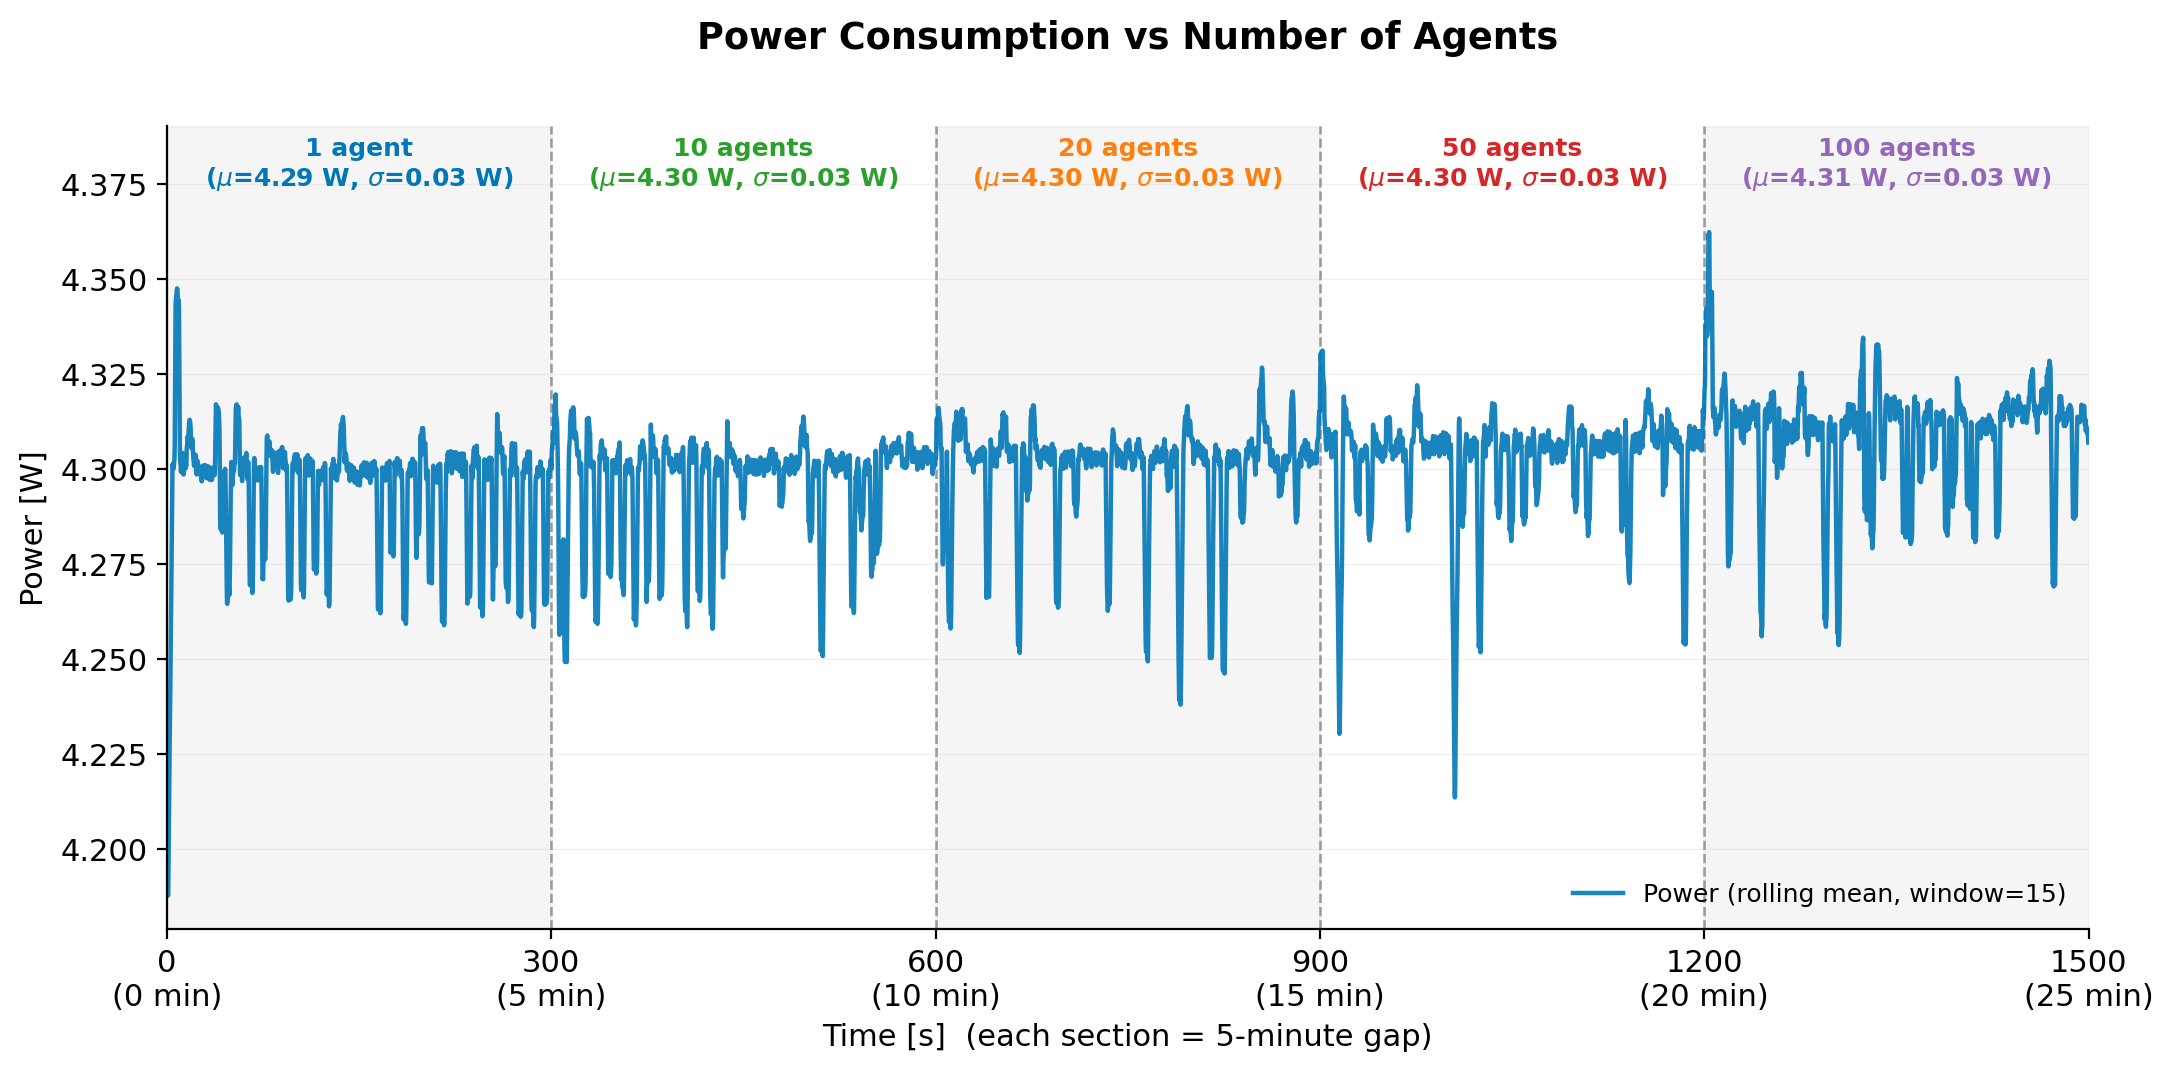
\includegraphics[width=0.85\linewidth]{power_agents.png}
\caption{Aggregate power consumption of the STM32MP257F-DK as the number of
co-located agents grows from $1$ to $100$, measured on the STM32MP257F-DK board.
The draw stays close to $4.3$~W, so the asynchronous communication layer adds no
measurable power overhead.}
\label{fig:power_agents}
\end{figure}

The base network traffic was tracked with the same scaling, all sensing agents
simulated on a single machine: a mock leader ran only the discovery and
tool-aggregation overlay (no model, election or dispatch) while the fleet grew from
$1$ to $100$. Table~\ref{tab:net_load} reports the leader's base traffic as bytes in
and out per minute (application-level JSON payload only, in KiB/min). The received
load grows linearly with the fleet and is dominated by discovery: each agent
re-announces every two seconds, so the HELLO beacons add about $1.8$~KiB/min per
agent, reaching $184.8$~KiB/min in and only $10.5$~KiB/min out at $100$ agents. Even
then the payload is a few hundred KiB per minute, so the network is not the
bottleneck and the leader language-model processing dominates the latency. The two
quantities that drive that processing, the number of exposed tools and the number of
aggregated replies, are studied next.

% Leader network-load table. Extracted from network.tex (generated by
% aggregate_network.py). Sourced from graphs/ and \input into latency.tex.
\begin{table}[H]
\centering
\caption{Leader base network load as the number of sensing agents grows, all agents
simulated on a single machine. Rates are bytes in and out per minute, averaged over
the one-minute hold at each fleet size (window length in the second column); the
idle row is the leader alone after the fleet stopped. Application-level JSON payload
only (KiB/min), excluding TCP/IP/Ethernet and handshake overhead.}
\label{tab:net_load}
\begin{tabular}{cccccc}
\toprule
\textbf{Agents} & \textbf{Window [s]} & \textbf{Msgs/min in} & \textbf{Msgs/min out} & \textbf{In [KiB/min]} & \textbf{Out [KiB/min]} \\
\midrule
0 (idle) & 431 & 30 & 30 & 1.7 & 1.7 \\
1 & 60 & 76 & 40 & 5.9 & 2.6 \\
10 & 60 & 351 & 43 & 22.5 & 2.8 \\
20 & 60 & 642 & 62 & 36.8 & 4.5 \\
50 & 60 & 1578 & 81 & 96.2 & 6.2 \\
100 & 60 & 2833 & 130 & 184.8 & 10.5 \\
\bottomrule
\end{tabular}
\end{table}


\subsection{Latency as the number of tools grows}
\label{subsub:latency:tools}

In this experiment the leader is presented with a growing pool of tools
($1$, $6$, $12$, $18$ and $24$) while a single sensing agent returns one result per
query; ten queries whose ground-truth tool is \texttt{detect\_people} are issued at
each pool size. Dispatch-stage statistics are computed over all ten queries, and
reply-stage and end-to-end statistics over the queries that produced a tool result
(their count $n$ is reported), because a missed or abstained call terminates the
pipeline after dispatch. Table~\ref{tab:lat_qwen} reports \texttt{Qwen3:1.7b} on
the Hailo and Table~\ref{tab:lat_fgemma} \texttt{functiongemma:270m} on the STM32
CPU, both with the full prompt and no key-value (KV) cache reuse. The end-to-end
time is decomposed into three stages whose per-query sum it equals: the dispatch
stage query$\rightarrow$tool, the sensing turnaround tool$\rightarrow$result, and
the answer stage result$\rightarrow$reply. Each end-to-end value is measured per
query and then averaged, so the three stage columns add up to the E2E column. The
tool$\rightarrow$result stage is the sensing agent's turnaround: the time from the
leader issuing the tool call to receiving the result over the real TCP network (a
\texttt{net.dispatch} round trip), including the skill execution on the other board.
It reflects where the sensing agent runs: in the Qwen3 configuration the tool
executes on the STM32 (YOLOv8n person detection on the CPU), so
tool$\rightarrow$result is about $0.6$~s, whereas in the functiongemma configuration
it executes on the Raspberry Pi 5 (YOLOv8n on the Hailo NPU), about $0.05$~s. The
dispatch prompt embeds the full JSON schema of every exposed tool, so it lengthens
by about $47$ tokens per tool for Qwen3 ($223$ to $1318$ tokens) and about $29$ for
functiongemma ($97$ to $755$ tokens), whereas the reply prompt never carries the
tool list and stays constant ($208$ and $165$ tokens respectively); the standard
pipeline also swaps the system prompt between the two stages, so each prefills
independently. The prefill of this growing dispatch prompt (the dispatch TTFT) is
the dominant, growing part of query$\rightarrow$tool and is plotted against the
prompt length in Figure~\ref{fig:ttft}.

\begin{table}[H]
\centering
\caption{Leader latency of \texttt{Qwen3:1.7b} on the Hailo-10H as the number of
exposed tools grows (sensing agent on the STM32, YOLOv8n on the CPU). Values are
mean $\pm$ standard deviation. The three stage columns sum to the end-to-end column,
which is the mean over the completed queries of their per-query total. Reply-stage
and E2E values at $6$ tools rest on the single query that dispatched correctly at
that pool size.}
\label{tab:lat_qwen}
\small
\begin{tabular}{cccccc}
\toprule
\textbf{Tools} & \textbf{Tokens in} & \textbf{Query$\rightarrow$tool [s]} & \textbf{Tool$\rightarrow$result [s]} & \textbf{Result$\rightarrow$reply [s]} & \textbf{E2E [s]} \\
\midrule
1 & 223 & 4.98 $\pm$ 0.00 & 0.64 $\pm$ 0.03 & 4.83 $\pm$ 0.52 & 10.44 $\pm$ 0.52 \\
6 & 458 & 6.21 $\pm$ 0.00 & 0.62 $\pm$ 0.00 & 4.98 $\pm$ 0.00 & 11.81 $\pm$ 0.00 \\
12 & 742 & 8.06 $\pm$ 0.00 & 0.64 $\pm$ 0.04 & 4.77 $\pm$ 0.51 & 13.47 $\pm$ 0.51 \\
18 & 1030 & 9.96 $\pm$ 0.13 & 0.61 $\pm$ 0.22 & 4.98 $\pm$ 0.81 & 15.55 $\pm$ 0.73 \\
24 & 1318 & 11.77 $\pm$ 0.00 & 0.63 $\pm$ 0.01 & 4.80 $\pm$ 0.54 & 17.19 $\pm$ 0.53 \\
\bottomrule
\end{tabular}
\end{table}

\begin{table}[H]
\centering
\caption{Leader latency of \texttt{functiongemma:270m} on the STM32 CPU (full
prompt, no KV cache reuse) as the number of exposed tools grows (sensing agent on
the Raspberry Pi 5, YOLOv8n on the Hailo NPU). Values are mean $\pm$ standard
deviation. The three stage columns sum to the end-to-end column, the mean over the
completed queries of their per-query total.}
\label{tab:lat_fgemma}
\small
\begin{tabular}{cccccc}
\toprule
\textbf{Tools} & \textbf{Tokens in} & \textbf{Query$\rightarrow$tool [s]} & \textbf{Tool$\rightarrow$result [s]} & \textbf{Result$\rightarrow$reply [s]} & \textbf{E2E [s]} \\
\midrule
1 & 97 & 9.12 $\pm$ 0.12 & 0.05 $\pm$ 0.00 & 17.62 $\pm$ 1.31 & 26.79 $\pm$ 1.40 \\
6 & 237 & 20.02 $\pm$ 0.12 & 0.05 $\pm$ 0.01 & 17.62 $\pm$ 1.30 & 37.69 $\pm$ 1.37 \\
12 & 407 & 36.94 $\pm$ 0.15 & 0.05 $\pm$ 0.00 & 17.49 $\pm$ 1.33 & 54.49 $\pm$ 1.44 \\
18 & 581 & 52.82 $\pm$ 0.16 & 0.07 $\pm$ 0.05 & 17.60 $\pm$ 1.31 & 70.50 $\pm$ 1.41 \\
24 & 755 & 69.42 $\pm$ 0.16 & 0.05 $\pm$ 0.00 & 17.50 $\pm$ 1.33 & 86.96 $\pm$ 1.45 \\
\bottomrule
\end{tabular}
\end{table}

A third configuration repeats the \texttt{functiongemma:270m} measurement with a
shorter, fixed dispatch prompt (of the form "You are a model that can do function
calling with the following functions") and KV-cache reuse across the ten queries of
each pool. The KV cache is reset whenever the number of tools changes, so the tool
descriptions are prefilled once per pool: the first query pays the full prefill and
the following nine reuse the cache, re-prefilling only the short user message.
Table~\ref{tab:lat_fgemma_kv} reports the same stage breakdown for this
configuration, over the nine warm (cached) queries of each pool; the one-time cold
first query of each pool is excluded here and reported in the TTFT comparison of
Table~\ref{tab:ttft_cmp}.

\begin{table}[H]
\centering
\caption{Leader latency of \texttt{functiongemma:270m} on the STM32 CPU with the
short prompt and KV-cache reuse (cache reset when the tool count changes). This run
dispatched to an in-place mock sensing agent, so tool$\rightarrow$result (about
$0.59$~s) reflects the mock turnaround rather than a physical device. Values are
mean $\pm$ standard deviation over the nine warm (cached) queries of each pool; the
cold first query is excluded (see Table~\ref{tab:ttft_cmp}). The three stage columns
sum to the end-to-end column.}
\label{tab:lat_fgemma_kv}
\small
\begin{tabular}{cccccc}
\toprule
\textbf{Tools} & \textbf{Tokens in} & \textbf{Query$\rightarrow$tool [s]} & \textbf{Tool$\rightarrow$result [s]} & \textbf{Result$\rightarrow$reply [s]} & \textbf{E2E [s]} \\
\midrule
1 & 88 & 2.45 $\pm$ 0.13 & 0.59 $\pm$ 0.00 & 6.74 $\pm$ 2.13 & 9.78 $\pm$ 2.14 \\
6 & 228 & 2.48 $\pm$ 0.13 & 0.59 $\pm$ 0.00 & 7.26 $\pm$ 1.97 & 10.33 $\pm$ 1.99 \\
12 & 398 & 2.68 $\pm$ 0.14 & 0.59 $\pm$ 0.00 & 7.50 $\pm$ 1.86 & 10.76 $\pm$ 1.84 \\
18 & 572 & 2.88 $\pm$ 0.15 & 0.59 $\pm$ 0.00 & 6.46 $\pm$ 1.30 & 9.93 $\pm$ 1.28 \\
24 & 746 & 2.99 $\pm$ 0.20 & 0.59 $\pm$ 0.00 & 7.51 $\pm$ 1.33 & 11.09 $\pm$ 1.34 \\
\bottomrule
\end{tabular}
\end{table}

Table~\ref{tab:ttft_cmp} collects the dispatch TTFT (the prompt prefill) of the
three configurations: \texttt{Qwen3:1.7b} on the Hailo, \texttt{functiongemma:270m}
with the full prompt and no reuse, and \texttt{functiongemma:270m} with the short
prompt and KV reuse, the last split into the cold first-load of each pool and the
warm cached queries. Table~\ref{tab:e2e} then compares the end-to-end latency of the
three, using the steady-state (cached) value for the KV configuration.

\begin{table}[H]
\centering
\caption{Dispatch TTFT [s] (prompt prefill, mean $\pm$ standard deviation) as the
number of exposed tools grows, for the three configurations. For the short-prompt KV
configuration the cold first-load of each pool and the warm cached queries are shown
separately; the cold column has no deviation as it is a single query per pool.}
\label{tab:ttft_cmp}
\begin{tabular}{ccccc}
\toprule
\textbf{Tools} & \textbf{Qwen3, Hailo [s]} & \textbf{functiongemma, no KV [s]} & \textbf{functiongemma KV, cold [s]} & \textbf{functiongemma KV, warm [s]} \\
\midrule
1 & 1.86 $\pm$ 0.00 & 7.67 $\pm$ 0.12 & 7.03 & 1.01 $\pm$ 0.13 \\
6 & 3.09 $\pm$ 0.00 & 18.56 $\pm$ 0.12 & 17.94 & 1.02 $\pm$ 0.13 \\
12 & 4.94 $\pm$ 0.00 & 35.40 $\pm$ 0.14 & 34.77 & 1.14 $\pm$ 0.14 \\
18 & 6.80 $\pm$ 0.00 & 51.20 $\pm$ 0.16 & 50.41 & 1.25 $\pm$ 0.15 \\
24 & 8.65 $\pm$ 0.00 & 67.79 $\pm$ 0.16 & 67.03 & 1.27 $\pm$ 0.15 \\
\bottomrule
\end{tabular}
\end{table}

\begin{table}[H]
\centering
\caption{End-to-end reply latency [s] (mean $\pm$ standard deviation) binned by the
number of exposed tools, for the three configurations. The KV-cache column reports
the steady-state (cached) latency. $^{*}$ single completed query at this pool size,
so no standard deviation is available.}
\label{tab:e2e}
\begin{tabular}{cccc}
\toprule
\textbf{Tools} & \textbf{Qwen3:1.7b, no KV [s]} & \textbf{functiongemma, no KV [s]} & \textbf{functiongemma, KV cache [s]} \\
\midrule
1 & 10.44 $\pm$ 0.52 & 26.79 $\pm$ 1.40 & 9.78 $\pm$ 2.14 \\
6 & 11.81$^{*}$ & 37.69 $\pm$ 1.37 & 10.33 $\pm$ 1.99 \\
12 & 13.47 $\pm$ 0.51 & 54.49 $\pm$ 1.44 & 10.76 $\pm$ 1.84 \\
18 & 15.55 $\pm$ 0.73 & 70.50 $\pm$ 1.41 & 9.93 $\pm$ 1.28 \\
24 & 17.19 $\pm$ 0.53 & 86.96 $\pm$ 1.45 & 11.09 $\pm$ 1.34 \\
\bottomrule
\end{tabular}
\end{table}

\begin{figure}[H]
\centering
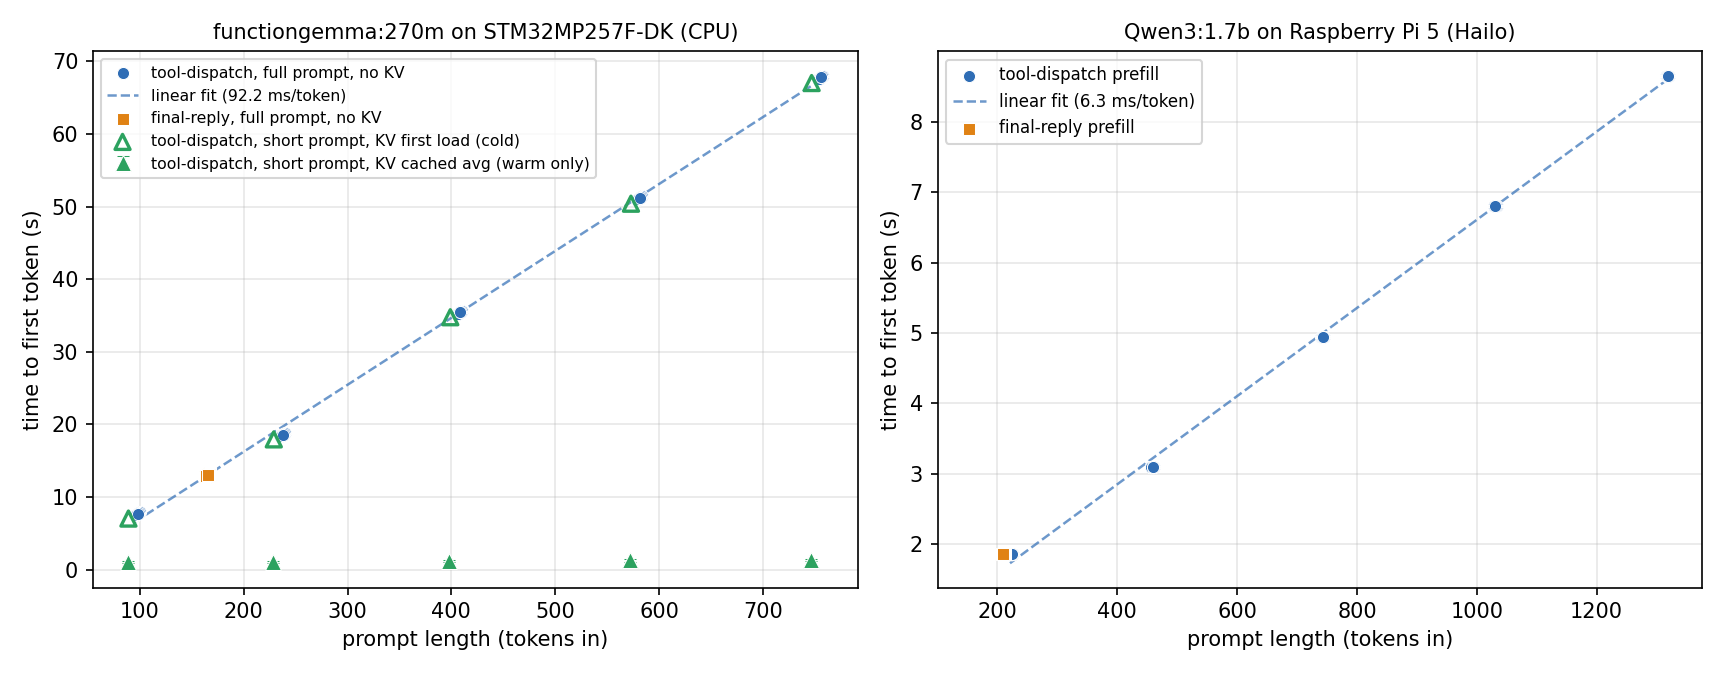
\includegraphics[width=\linewidth]{ttft_vs_tokens.png}
\caption{Time to first token (prefill time) against prompt length for the two
leader backends. Filled circles are the tool-dispatch stage with the full prompt
and no KV reuse; squares are the final-reply stage. On the STM32 panel, hollow
triangles are the cold first-load dispatch prefill of the short-prompt KV
configuration (one per pool, first query), and filled triangles are the same stage
averaged only over the warm cached queries of each pool, with error bars for the
standard deviation. The KV cache is reset at each change in the number of tools.
Dashed lines are least-squares fits through the full-prompt dispatch points.}
\label{fig:ttft}
\end{figure}

\subsection{Latency as the number of replies grows}
\label{subsub:latency:replies}

This experiment exposes a single tool and varies the number of sensing agents that
return a result ($1$, $5$, $10$, $15$, $20$), so the leader aggregates a growing set
of results into one reply; ten queries are issued at each setting. Three
configurations are compared: \texttt{Qwen3:1.7b} on the Hailo, and
\texttt{functiongemma:270m} on the STM32 CPU with and without KV-cache reuse of the
fixed prompt prefix (labelled KV reuse and reset, the reply-axis analogues of the
KV and no-KV tool-scaling configurations). As in the tool-scaling test, the
end-to-end time is decomposed into stages measured per query and averaged. The
sensing turnaround tool$\rightarrow$result is omitted here: the result set is
assembled in-process (the harness builds the exact result the dispatcher would
return, without the network hop, since the network latency is not the quantity under
study), so tool$\rightarrow$result only times that in-process construction and is
negligible (under $0.1$~ms), leaving query$\rightarrow$tool $+$
result$\rightarrow$reply $=$ E2E. In all three configurations the dispatch stage
(query$\rightarrow$tool) is essentially invariant (a single tool), whereas the
answer-stage prompt lengthens with the number of aggregated results and drives the
latency. Tables~\ref{tab:lat_replies}, \ref{tab:lat_replies_reset}
and~\ref{tab:lat_replies_kvreuse} give the per-stage breakdown for
\texttt{Qwen3:1.7b} on the Hailo, \texttt{functiongemma:270m} without KV reuse, and
\texttt{functiongemma:270m} with KV reuse; for Qwen3 the answer prompt grows from
$200$ to $553$ tokens and the end-to-end time from $8.64$~s to $11.09$~s.
Table~\ref{tab:replies_cmp} compares the answer-stage TTFT of the three
configurations, and Figure~\ref{fig:replies} plots it against the answer prompt
length.

\begin{table}[H]
\centering
\caption{Leader latency of \texttt{Qwen3:1.7b} on the Hailo as the number of
aggregated replies grows (single tool). Values are mean $\pm$ standard deviation
over ten queries. The two stage columns sum to E2E; tool$\rightarrow$result (the
in-process build of the reply set, no network hop) is negligible ($<0.1$~ms) and
omitted.}
\label{tab:lat_replies}
\small
\begin{tabular}{cccccc}
\toprule
\textbf{Replies} & \textbf{Answer tokens in} & \textbf{Answer tokens out} & \textbf{Query$\rightarrow$tool [s]} & \textbf{Result$\rightarrow$reply [s]} & \textbf{E2E [s]} \\
\midrule
1 & 200 & 8.8 & 4.96 $\pm$ 0.00 & 3.68 $\pm$ 0.29 & 8.64 $\pm$ 0.29 \\
5 & 272 & 21.6 & 4.96 $\pm$ 0.00 & 6.32 $\pm$ 2.04 & 11.28 $\pm$ 2.04 \\
10 & 363 & 11.1 & 4.96 $\pm$ 0.00 & 4.77 $\pm$ 1.18 & 9.73 $\pm$ 1.18 \\
15 & 458 & 13.9 & 4.96 $\pm$ 0.00 & 5.97 $\pm$ 1.52 & 10.93 $\pm$ 1.52 \\
20 & 553 & 11.7 & 4.96 $\pm$ 0.00 & 6.13 $\pm$ 1.05 & 11.09 $\pm$ 1.05 \\
\bottomrule
\end{tabular}
\end{table}

\begin{table}[H]
\centering
\caption{Leader latency of \texttt{functiongemma:270m} on the STM32 CPU without KV
reuse (\texttt{llm.reset()} before every generation, so each query is an independent
cold prefill) as the number of aggregated replies grows (single tool). Values are
mean $\pm$ standard deviation over ten queries; tool$\rightarrow$result is omitted as
above, so query$\rightarrow$tool $+$ result$\rightarrow$reply $=$ E2E.}
\label{tab:lat_replies_reset}
\small
\begin{tabular}{cccccc}
\toprule
\textbf{Replies} & \textbf{Answer tokens in} & \textbf{Answer tokens out} & \textbf{Query$\rightarrow$tool [s]} & \textbf{Result$\rightarrow$reply [s]} & \textbf{E2E [s]} \\
\midrule
1 & 161 & 17.2 & 9.11 $\pm$ 0.12 & 16.23 $\pm$ 0.99 & 25.34 $\pm$ 1.06 \\
5 & 233 & 30.8 & 9.12 $\pm$ 0.12 & 24.80 $\pm$ 4.50 & 33.91 $\pm$ 4.52 \\
10 & 324 & 44.9 & 9.11 $\pm$ 0.12 & 38.08 $\pm$ 6.94 & 47.19 $\pm$ 7.02 \\
15 & 419 & 106.6 & 9.11 $\pm$ 0.13 & 60.93 $\pm$ 38.10 & 70.04 $\pm$ 38.08 \\
20 & 514 & 71.8 & 9.10 $\pm$ 0.12 & 61.38 $\pm$ 24.10 & 70.48 $\pm$ 24.11 \\
\bottomrule
\end{tabular}
\end{table}

\begin{table}[H]
\centering
\caption{Leader latency of \texttt{functiongemma:270m} on the STM32 CPU with
KV-cache reuse (the cache is never reset across the run) as the number of aggregated
replies grows (single tool). Values are mean $\pm$ standard deviation over ten
queries; tool$\rightarrow$result is omitted as above. Only the run's first query, in
the $1$-reply row, pays a cold prefill, which raises that row's
query$\rightarrow$tool mean and spread; all later queries reuse the cache.}
\label{tab:lat_replies_kvreuse}
\small
\begin{tabular}{cccccc}
\toprule
\textbf{Replies} & \textbf{Answer tokens in} & \textbf{Answer tokens out} & \textbf{Query$\rightarrow$tool [s]} & \textbf{Result$\rightarrow$reply [s]} & \textbf{E2E [s]} \\
\midrule
1 & 125 & 14.9 & 3.06 $\pm$ 1.91 & 5.54 $\pm$ 1.63 & 8.60 $\pm$ 2.86 \\
5 & 197 & 53.2 & 2.46 $\pm$ 0.12 & 19.26 $\pm$ 6.83 & 21.72 $\pm$ 6.83 \\
10 & 288 & 53.7 & 2.45 $\pm$ 0.12 & 28.59 $\pm$ 8.61 & 31.05 $\pm$ 8.66 \\
15 & 383 & 102.9 & 2.46 $\pm$ 0.12 & 48.00 $\pm$ 19.41 & 50.46 $\pm$ 19.41 \\
20 & 478 & 155.4 & 2.46 $\pm$ 0.12 & 69.00 $\pm$ 30.66 & 71.46 $\pm$ 30.69 \\
\bottomrule
\end{tabular}
\end{table}

\begin{table}[H]
\centering
\caption{Answer-stage TTFT [s] (mean $\pm$ standard deviation) as the number of
aggregated replies grows, for the three configurations. functiongemma is measured
without KV reuse (reset) and with KV reuse of the fixed prompt prefix.}
\label{tab:replies_cmp}
\begin{tabular}{cccc}
\toprule
\textbf{Replies} & \textbf{Qwen3:1.7b, Hailo [s]} & \textbf{functiongemma, reset [s]} & \textbf{functiongemma, KV reuse [s]} \\
\midrule
1 & 1.85 $\pm$ 0.00 & 12.65 $\pm$ 0.12 & 2.46 $\pm$ 0.01 \\
5 & 1.86 $\pm$ 0.00 & 18.24 $\pm$ 0.12 & 8.04 $\pm$ 0.02 \\
10 & 2.47 $\pm$ 0.00 & 28.21 $\pm$ 0.12 & 16.83 $\pm$ 0.02 \\
15 & 3.09 $\pm$ 0.00 & 36.42 $\pm$ 0.13 & 25.07 $\pm$ 0.04 \\
20 & 3.71 $\pm$ 0.00 & 44.78 $\pm$ 0.18 & 33.28 $\pm$ 0.02 \\
\bottomrule
\end{tabular}
\end{table}

\begin{figure}[H]
\centering
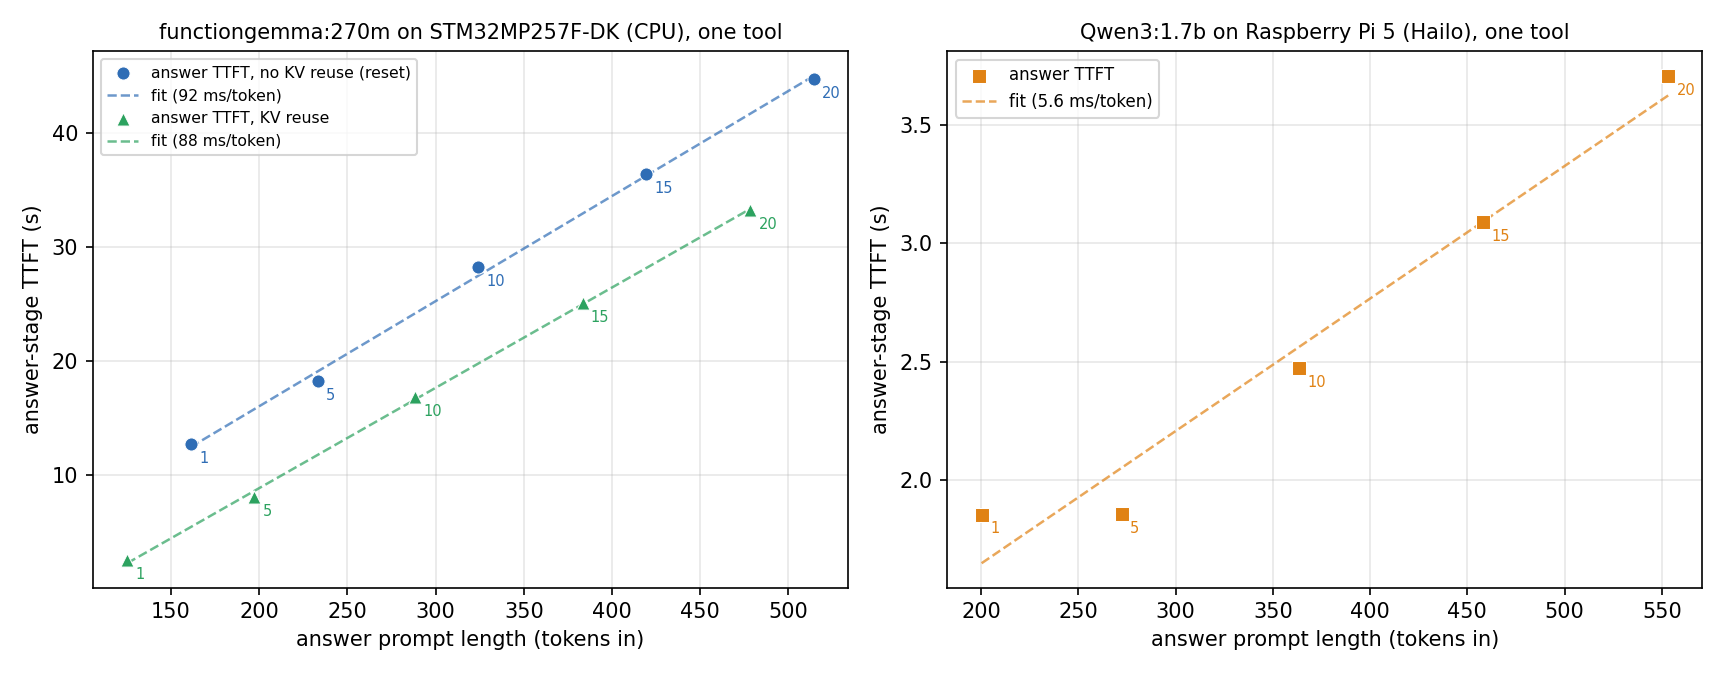
\includegraphics[width=\linewidth]{latency_vs_replies.png}
\caption{Answer-stage TTFT (final-reply prefill) against the answer prompt length
for a single tool and a growing number of aggregated replies. Left: functiongemma
on the STM32 CPU, without KV reuse (reset, circles) and with KV reuse (triangles).
Right: Qwen3:1.7b on the Hailo. The number of aggregated replies is annotated on
each point; dashed lines are least-squares fits. On the STM32 the two lines are
nearly parallel: KV reuse lowers the intercept by a fixed amount but leaves the
per-token slope unchanged.}
\label{fig:replies}
\end{figure}

\subsection{Discussion}
\label{subsec:latency_discussion}

The agent-scaling measurements confirm that the network overhead is not impactful in
the test performed: up to $100$ simulated agents the leader's traffic stays at a few
hundred KiB per minute (Table~\ref{tab:net_load}) and the power near $4.3$~W
(Table~\ref{tab:power_agents}). The end-to-end latency is instead governed by
prefill. In the
tool-scaling experiment almost all of the end-to-end growth is concentrated in the
dispatch stage: the query$\rightarrow$tool time inflates with the tool count while
tool$\rightarrow$result and result$\rightarrow$reply stay flat
(Tables~\ref{tab:lat_qwen} and~\ref{tab:lat_fgemma}), and Figure~\ref{fig:ttft} shows
that its prefill (the dispatch TTFT) rises linearly with the prompt length on both
devices, at about $92$~ms per token on the STM32 CPU against only $6.3$~ms per token
on the Hailo, a factor of roughly $14$. The same law governs the answer stage on the reply axis, where the
answer TTFT grows at about $90$~ms per token on the STM32 and $5.6$~ms per token on
the Hailo (Figure~\ref{fig:replies}), matching the dispatch rates. The accelerator
is therefore the single most important factor in meeting the latency target.

The two scaling axes load different stages and are essentially independent. Adding
tools lengthens only the dispatch prompt: the query$\rightarrow$tool stage grows
while the result$\rightarrow$reply stage stays flat around $4.8$~s
(Table~\ref{tab:lat_qwen}). Adding replies lengthens only the answer prompt: the
query$\rightarrow$tool stage stays constant while result$\rightarrow$reply grows
(Table~\ref{tab:lat_replies}). Because the dispatch cost depends on the
number of tools and not on how many agents expose them, a network of $24$ agents
each exposing one tool and a single agent exposing $24$ tools impose the same
dispatch load, on top of which the reply-aggregation cost adds. The two costs are
additive, which makes the leader latency predictable from the tool count and the
expected number of responders.

Under these conditions \texttt{Qwen3:1.7b} on the Hailo satisfies the $20$~s
responsiveness requirement across the whole range tested: at most $17.19$~s with
$24$ tools (Table~\ref{tab:lat_qwen}) and at most $11.09$~s with $20$ aggregated
replies (Table~\ref{tab:lat_replies}). \texttt{functiongemma:270m} on the STM32 CPU
does not, on either axis: with the full prompt it needs $26.79$~s already with a
single tool and reaches $86.96$~s with $24$ (Table~\ref{tab:lat_fgemma}), and on the
reply axis its answer TTFT alone reaches $44.78$~s at $20$ replies
(Table~\ref{tab:replies_cmp}). On a microprocessor-class leader the number of
exposed tools and the number of responders are therefore first-class design
parameters.

The KV cache helps less than it first appears, and the reply-scaling experiment
shows why. With a shorter, fixed prompt, KV reuse removes almost the entire
tool-description prefill for repeated queries, collapsing the dispatch TTFT from tens
of seconds to about $1$~s (Table~\ref{tab:ttft_cmp}) and bringing functiongemma back under
budget in steady state on the tool axis (Table~\ref{tab:e2e}). However, this saving
is a fixed offset, not a per-token reduction. On the reply axis the two
functiongemma answer-TTFT curves, with and without reuse, are nearly parallel (about
$90$~ms per token in both cases, Figure~\ref{fig:replies}): reuse only caches the
fixed prompt prefix, lowering the intercept by roughly $10$~s, while the aggregated
results, which differ on every query, must still be prefilled. The absolute saving
therefore stays roughly constant as the answer prompt grows, so its relative benefit
shrinks from about $80\%$ at one reply ($2.46$ against $12.65$~s) to about $26\%$ at
twenty ($33.28$ against $44.78$~s, Table~\ref{tab:replies_cmp}). Two further limits
apply on the tool axis: the cold first query of every context still pays the full
prefill, from $7.03$~s to $67.03$~s (Table~\ref{tab:ttft_cmp}), reset whenever the tool set
changes, and the prompt swap between the dispatch and reply stages discards the
dispatch cache before the answer is generated. KV reuse thus removes a fixed part of
the prefill but not its growth with either tools or replies.

Finally, on the reply axis the end-to-end variance is driven by the generated reply
length rather than the input. The answer TTFT is highly reproducible (standard
deviation below $2$~ms), but the result-to-reply and end-to-end times vary by
$1$ to $2$~s (Table~\ref{tab:lat_replies}) because the number of generated tokens
fluctuates: the five-reply case produced the longest replies ($21.6$ output tokens
on average) and the largest spread. Once the prefill cost is bounded, controlling the
output length is the main lever for tightening tail latency.

\end{document}
